\documentclass[tikz]{standalone}
\usepackage{tikz}
\usetikzlibrary{calc}
\usetikzlibrary{positioning}
\usetikzlibrary{fit}
\usetikzlibrary{backgrounds}

\definecolor{lightGreen}{HTML}{d5e8d4}
\definecolor{lightYellow}{HTML}{fff2cc}
\definecolor{lightGray}{HTML}{f5f5f5}
\definecolor{lightRed}{HTML}{ff9999}
\definecolor{lightBlue}{HTML}{d5e5fc}
\definecolor{lightCyan}{HTML}{a7dfe3}
\pgfdeclarelayer{main_bg}
\pgfdeclarelayer{back_bg}
\pgfsetlayers{main_bg,back_bg,main}

\newcommand{\metarect}[7]{
    \begin{scope}
        \node (#1) [rectangle, draw, text width=\rectWidth, minimum width=\rectWidth, minimum height=\rectHeight, #7] {};
        \node (#1_upper) [rectangle, draw, fill=#6, text width=\rectWidth, minimum width=\rectWidth, minimum height=\rectHeight*0.5, below=0.0pt of #1.north, anchor=north] {#2};
        \node (#1_middle) [rectangle, draw, fill=white, font=\tiny, text width=\rectWidth, minimum width=\rectWidth, minimum height=\rectHeight*0.25, below=-\the\pgflinewidth of #1_upper] {#3};
        \node (#1_bleft) [rectangle, draw, fill=white, font=\tiny, text width=\rectWidth*0.35, minimum width=\rectWidth*0.35, minimum height=\rectHeight*0.25, below=-\the\pgflinewidth of #1_middle.south west, anchor=north west] {#4};
        \node (#1_bright) [rectangle, draw, fill=white, font=\tiny, text width=\rectWidth*0.65, minimum width=\rectWidth*0.65, minimum height=\rectHeight*0.25, right=-\the\pgflinewidth of #1_bleft] {#5};
    \end{scope}
}

\newcommand{\metarectvec}[5]{
    \begin{scope}
        \node (#1) [draw, rectangle, text width=\rectWidth, minimum width=\rectWidth, minimum height=\rectHeight*0.25, #5] {};
        \node (#1_left) [draw, rectangle, fill=#4, font=\footnotesize, text width=\rectWidth*0.4, minimum width=\rectWidth*0.4, minimum height=\rectHeight*0.25, below=0.0pt of #1.north west, anchor=north west] {#2};
        \node (#1_right) [draw, rectangle, fill=white, font=\tiny, text width=\rectWidth*0.6, minimum width=\rectWidth*0.6, minimum height=\rectHeight*0.25, right=-\the\pgflinewidth of #1_left] {#3};
    \end{scope}
}

\begin{document}
    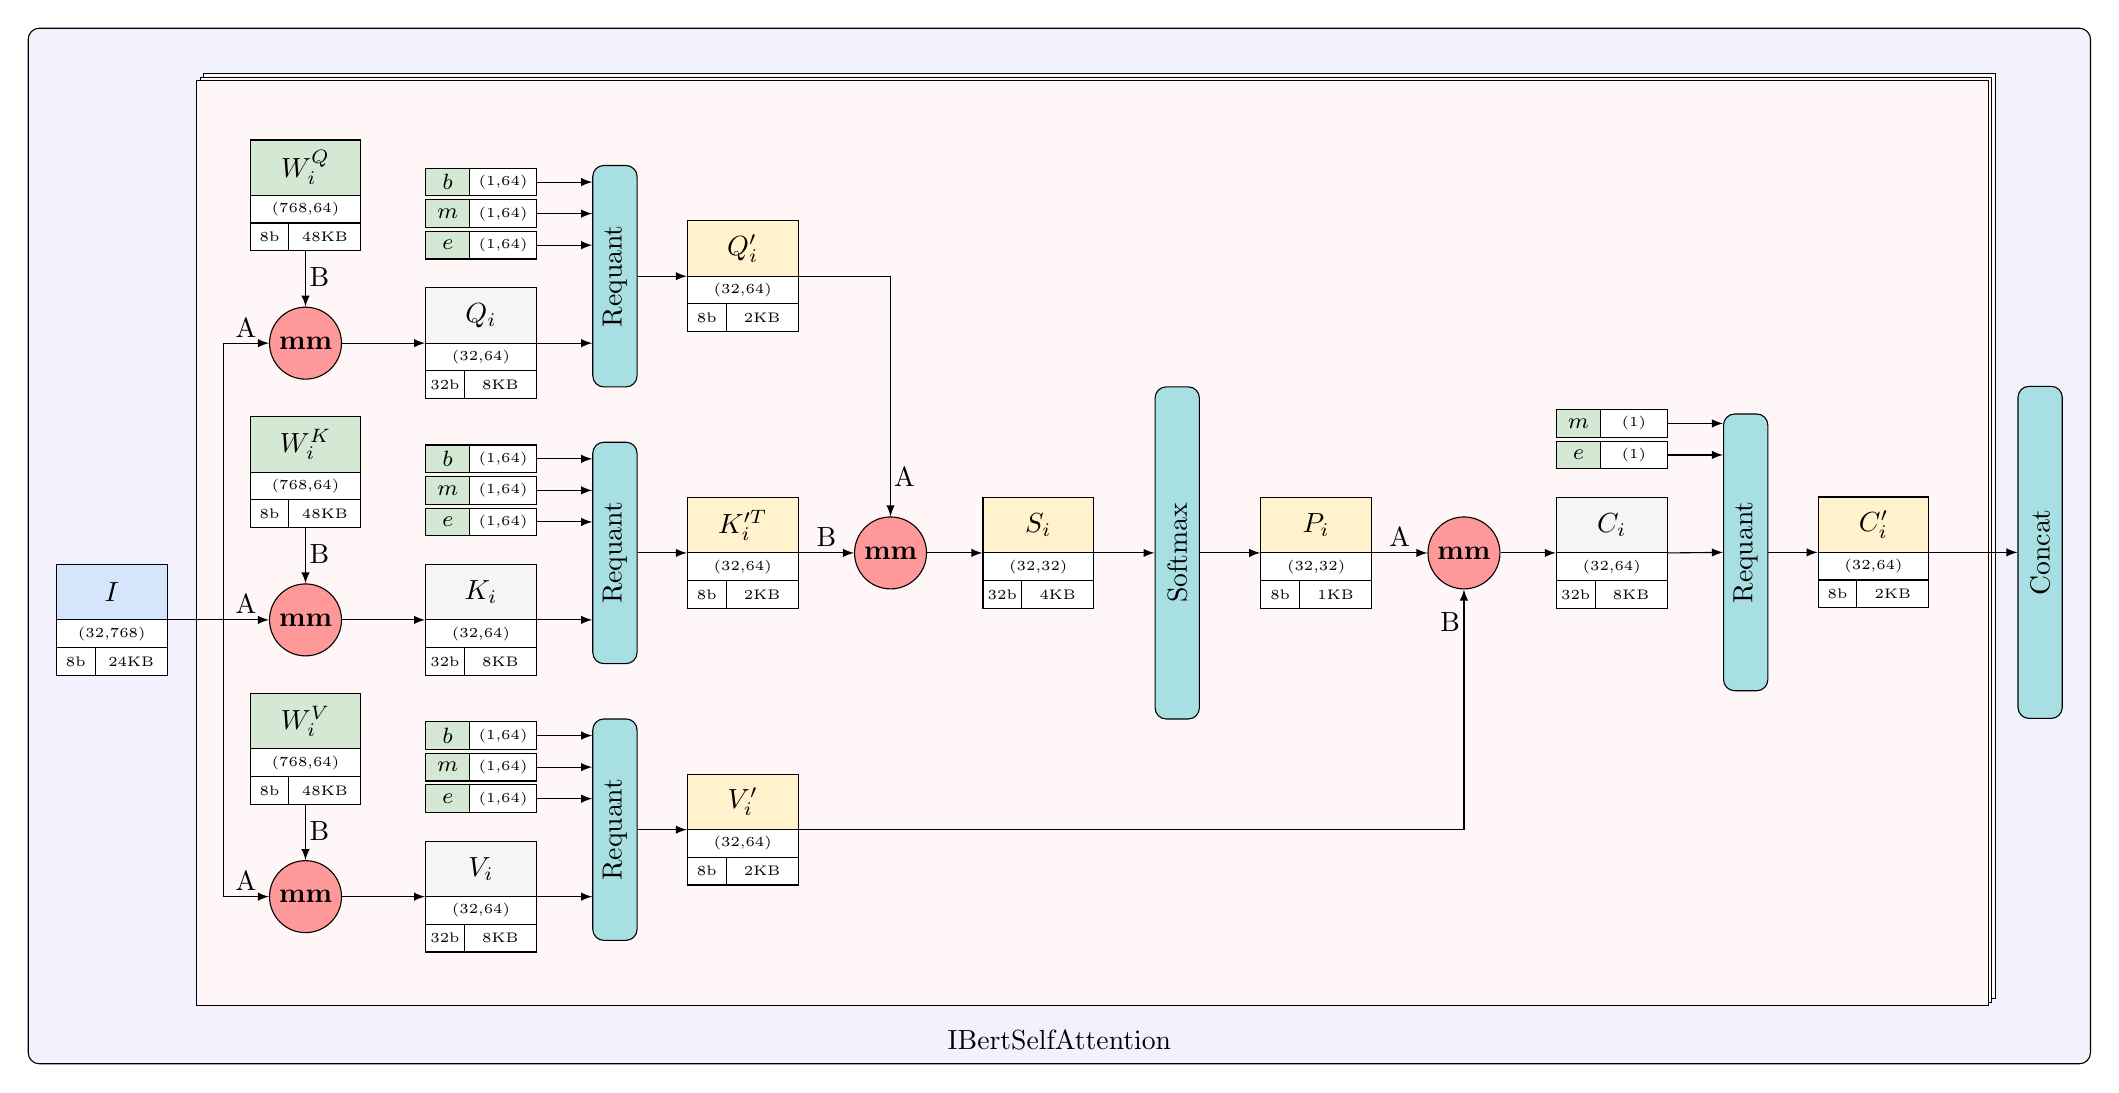
\begin{tikzpicture}[inner sep=0.0 pt, align=center]
    \pgfmathsetmacro{\rectWidth}{40}
    \pgfmathsetmacro{\rectHeight}{40}

    \metarect{layer_input}{$I$}{(32,768)}{8b}{24KB}{lightBlue}{}

    \pgfmathsetmacro{\multSize}{26 pt}
    \node [draw, circle, fill=lightRed, minimum size=\multSize, right=\rectWidth*1.75pt of layer_input.center, anchor=center] (mult1) {\textbf{mm}};
    \node [draw, circle, fill=lightRed, minimum size=\multSize, above=\rectHeight*2.5pt of mult1.center, anchor=center] (mult2) {\textbf{mm}};
    \node [draw, circle, fill=lightRed, minimum size=\multSize, below=\rectHeight*2.5pt of mult1.center, anchor=center] (mult3) {\textbf{mm}};

    \metarect{weight_Q}{$W_i^Q$}{(768,64)}{8b}{48KB}{lightGreen}{above=\rectHeight*0.5pt of mult2}
    \metarect{weight_K}{$W_i^K$}{(768,64)}{8b}{48KB}{lightGreen}{above=\rectHeight*0.5pt of mult1}
    \metarect{weight_V}{$W_i^V$}{(768,64)}{8b}{48KB}{lightGreen}{above=\rectHeight*0.5pt of mult3}

    \draw [-latex] (weight_Q.south) -- (mult2.north) node[near end, above, yshift=2pt, xshift=5pt] {B};
    \draw [-latex] (weight_K.south) -- (mult1.north) node[near end, above, yshift=2pt, xshift=5pt] {B};
    \draw [-latex] (weight_V.south) -- (mult3.north) node[near end, above, yshift=2pt, xshift=5pt] {B};

    \draw [-latex] (layer_input.east) -| ([xshift=\rectWidth*0.5 pt]layer_input.east) |- (mult2.west) node[near end, above, yshift=2pt] {A};
    \draw [-latex] (layer_input.east) -| ([xshift=\rectWidth*0.5 pt]layer_input.east) |- (mult1.west) node[near end, above, yshift=2pt] {A};
    \draw [-latex] (layer_input.east) -| ([xshift=\rectWidth*0.5 pt]layer_input.east) |- (mult3.west) node[near end, above, yshift=2pt] {A};

    \metarect{mixQ32b}{$Q_i$}{(32,64)}{32b}{8KB}{lightGray}{right=\rectWidth*0.75pt of mult2}
    \metarect{mixK32b}{$K_i$}{(32,64)}{32b}{8KB}{lightGray}{right=\rectWidth*0.75pt of mult1}
    \metarect{mixV32b}{$V_i$}{(32,64)}{32b}{8KB}{lightGray}{right=\rectWidth*0.75pt of mult3}

    \draw [-latex] (mult2.east) -- (mixQ32b.west);
    \draw [-latex] (mult1.east) -- (mixK32b.west);
    \draw [-latex] (mult3.east) -- (mixV32b.west);

    % \node [draw, rectangle, fill=lightGreen, font=\footnotesize, text width=\rectWidth, minimum width=\rectWidth, minimum height=\rectHeight*0.2, above=\rectHeight*0.25pt of mixQ32b.north] (qreq_e) {$e$};
    % \node [draw, rectangle, fill=lightGreen, font=\footnotesize, text width=\rectWidth, minimum width=\rectWidth, minimum height=\rectHeight*0.2, above=1.0pt of qreq_e.north] (qreq_m) {$m$};
    % \node [draw, rectangle, fill=lightGreen, font=\footnotesize, text width=\rectWidth, minimum width=\rectWidth, minimum height=\rectHeight*0.2, above=1.0pt of qreq_m.north] (qbias) {$b$};

    \metarectvec{qreq_e}{$e$}{(1,64)}{lightGreen}{above=\rectHeight*0.25pt of mixQ32b.north}
    \metarectvec{qreq_m}{$m$}{(1,64)}{lightGreen}{above=1.0pt of qreq_e.north}
    \metarectvec{qbias}{$b$}{(1,64)}{lightGreen}{above=1.0pt of qreq_m.north}
    
    % \node [draw, rectangle, fill=lightGreen, font=\footnotesize, text width=\rectWidth, minimum width=\rectWidth, minimum height=\rectHeight*0.2, above=\rectHeight*0.25pt of mixK32b.north] (kreq_e) {$e$};
    % \node [draw, rectangle, fill=lightGreen, font=\footnotesize, text width=\rectWidth, minimum width=\rectWidth, minimum height=\rectHeight*0.2, above=1.0pt of kreq_e.north] (kreq_m) {$m$};
    % \node [draw, rectangle, fill=lightGreen, font=\footnotesize, text width=\rectWidth, minimum width=\rectWidth, minimum height=\rectHeight*0.2, above=1.0pt of kreq_m.north] (kbias) {$b$};

    \metarectvec{kreq_e}{$e$}{(1,64)}{lightGreen}{above=\rectHeight*0.25pt of mixK32b.north}
    \metarectvec{kreq_m}{$m$}{(1,64)}{lightGreen}{above=1.0pt of kreq_e.north}
    \metarectvec{kbias}{$b$}{(1,64)}{lightGreen}{above=1.0pt of kreq_m.north}

    % \node [draw, rectangle, fill=lightGreen, font=\footnotesize, text width=\rectWidth, minimum width=\rectWidth, minimum height=\rectHeight*0.2, above=\rectHeight*0.25pt of mixV32b.north] (vreq_e) {$e$};
    % \node [draw, rectangle, fill=lightGreen, font=\footnotesize, text width=\rectWidth, minimum width=\rectWidth, minimum height=\rectHeight*0.2, above=1.0pt of vreq_e.north] (vreq_m) {$m$};
    % \node [draw, rectangle, fill=lightGreen, font=\footnotesize, text width=\rectWidth, minimum width=\rectWidth, minimum height=\rectHeight*0.2, above=1.0pt of vreq_m.north] (vbias) {$b$};

    \metarectvec{vreq_e}{$e$}{(1,64)}{lightGreen}{above=\rectHeight*0.25pt of mixV32b.north}
    \metarectvec{vreq_m}{$m$}{(1,64)}{lightGreen}{above=1.0pt of vreq_e.north}
    \metarectvec{vbias}{$b$}{(1,64)}{lightGreen}{above=1.0pt of vreq_m.north}

    \node [draw, fill=lightCyan, rounded corners, minimum width=\rectHeight*2, minimum height=\rectWidth*0.4, rotate=90, above right=\rectWidth*0.1pt and \rectWidth*0.5pt of mixQ32b, anchor=north] (reqQ) {Requant};
    \node [draw, fill=lightCyan, rounded corners, minimum width=\rectHeight*2, minimum height=\rectWidth*0.4, rotate=90, above right=\rectWidth*0.1pt and \rectWidth*0.5pt of mixK32b, anchor=north] (reqK) {Requant};
    \node [draw, fill=lightCyan, rounded corners, minimum width=\rectHeight*2, minimum height=\rectWidth*0.4, rotate=90, above right=\rectWidth*0.1pt and \rectWidth*0.5pt of mixV32b, anchor=north] (reqV) {Requant};

    \draw [-latex] (qreq_e.east) to[out=0,in=180] (reqQ.north |- qreq_e);
    \draw [-latex] (qreq_m.east) to[out=0,in=180] (reqQ.north |- qreq_m);
    \draw [-latex] (qbias.east) to[out=0,in=180] (reqQ.north |- qbias);

    \draw [-latex] (kreq_e.east) to[out=0,in=180] (reqK.north |- kreq_e);
    \draw [-latex] (kreq_m.east) to[out=0,in=180] (reqK.north |- kreq_m);
    \draw [-latex] (kbias.east) to[out=0,in=180] (reqK.north |- kbias);

    \draw [-latex] (vreq_e.east) to[out=0,in=180] (reqV.north |- vreq_e);
    \draw [-latex] (vreq_m.east) to[out=0,in=180] (reqV.north |- vreq_m);
    \draw [-latex] (vbias.east) to[out=0,in=180] (reqV.north |- vbias);
    
    \draw [-latex] (mixQ32b.east) to[out=0,in=180] (reqQ.north |- mixQ32b);
    \draw [-latex] (mixK32b.east) to[out=0,in=180] (reqK.north |- mixK32b);
    \draw [-latex] (mixV32b.east) to[out=0,in=180] (reqV.north |- mixV32b);


    \metarect{mixQ8b}{$Q_i'$}{(32,64)}{8b}{2KB}{lightYellow}{right=\rectWidth*0.65pt of reqQ.center}
    \metarect{mixK8b}{$K_i'^T$}{(32,64)}{8b}{2KB}{lightYellow}{right=\rectWidth*0.65pt of reqK.center}
    \metarect{mixV8b}{$V_i'$}{(32,64)}{8b}{2KB}{lightYellow}{right=\rectWidth*0.65pt of reqV.center}

    \draw [-latex] (reqQ.south) -- (mixQ8b.west);
    \draw [-latex] (reqK.south) -- (mixK8b.west);
    \draw [-latex] (reqV.south) -- (mixV8b.west);

    \node [draw, circle, fill=lightRed, minimum size=\multSize, right=\rectWidth*0.5pt of mixK8b] (multSelf1) {\textbf{mm}};
    \metarect{Si}{$S_i$}{(32,32)}{32b}{4KB}{lightYellow}{right=\rectWidth*0.5pt of multSelf1}

    \draw [-latex] (mixQ8b.east) -| (multSelf1.north) node[pos=0.95, above, xshift=5pt, yshift=2pt] {A};
    \draw [-latex] (mixK8b.east) -- (multSelf1.west) node[near end, above, xshift=-5pt, yshift=2pt] {B};
    \draw [-latex] (multSelf1.east) -- (Si.west);

    \node [draw, fill=lightCyan, rounded corners, minimum width=\rectHeight*3, minimum height=\rectWidth*0.4, rotate=90, right=\rectWidth*0.75pt of Si, anchor=center] (softmax) {Softmax};

    \metarect{Pi}{$P_i$}{(32,32)}{8b}{1KB}{lightYellow}{right=\rectWidth*0.75pt of softmax.center}
    \node [draw, circle, fill=lightRed, minimum size=\multSize, right=\rectWidth*0.5pt of Pi] (multSelf2) {\textbf{mm}};
    \metarect{Ci}{$C_i$}{(32,64)}{32b}{8KB}{lightGray}{right=\rectWidth*0.5pt of multSelf2}
    \node [draw, fill=lightCyan, rounded corners, minimum width=\rectHeight*2.5, minimum height=\rectWidth*0.4, rotate=90, above right=-\rectWidth*0.5pt and \rectWidth*0.5pt of Ci, anchor=north] (reqC) {Requant};
    \metarect{Ci8b}{$C_i'$}{(32,64)}{8b}{2KB}{lightYellow}{right=\rectWidth*0.65pt of reqC.center}

    % \node [draw, rectangle, fill=lightGreen, font=\footnotesize, text width=\rectWidth, minimum width=\rectWidth, minimum height=\rectHeight*0.2, above=\rectHeight*0.25pt of Ci.north] (creq_e) {$e$};
    % \node [draw, rectangle, fill=lightGreen, font=\footnotesize, text width=\rectWidth, minimum width=\rectWidth, minimum height=\rectHeight*0.2, above=1.0pt of creq_e.north] (creq_m) {$m$};

    \metarectvec{creq_e}{$e$}{(1)}{lightGreen}{above=\rectHeight*0.25pt of Ci.north}
    \metarectvec{creq_m}{$m$}{(1)}{lightGreen}{above=1.0pt of creq_e.north}

    \draw [-latex] (creq_e.east) to[out=0,in=180] (reqC.north |- creq_e);
    \draw [-latex] (creq_m.east) to[out=0,in=180] (reqC.north |- creq_m);
    % \draw [-latex] (Ci.east) to[out=0,in=180] (reqC.north |- Ci);

    \draw [-latex] (Si.east) -- (softmax.north);
    \draw [-latex] (softmax.south) -- (Pi.west);
    \draw [-latex] (Pi.east) -- (multSelf2.west) node[near end, above, xshift=-5pt, yshift=2pt] {A};
    
    \draw [-latex] (mixV8b.east) -| (multSelf2.south) node[pos=0.9, above, xshift=-5pt, yshift=2pt] {B};
    \draw [-latex] (multSelf2.east) -- (Ci.west);
    \draw [-latex] (reqC.south) -- (Ci8b.west);
    \draw [-latex] (Ci.east) -- (reqC.north);

    \begin{pgfonlayer}{main_bg}
        \node (self_rect) [draw, rectangle, fill=black!3, inner sep=20pt, fit=(weight_Q)(weight_K)(weight_V)(mixQ32b)(mixV32b)(Ci8b)(reqQ)(reqK)(reqV)] {};
        \begin{pgfonlayer}{back_bg}
            \foreach \x in {3,...,1} {
                \node [draw, rectangle, fill=red!3, fit=(self_rect), above right=\x*1.25pt-\the\pgflinewidth and \x*1.25pt-\the\pgflinewidth of self_rect.south west] {};
            }
        \end{pgfonlayer}
    \end{pgfonlayer}

    \node [draw, fill=lightCyan, rounded corners, minimum width=\rectHeight*3, minimum height=\rectWidth*0.4, rotate=90, right=\rectWidth*1pt of Ci8b, anchor=center] (concat) {Concat};
    \draw [-latex] (Ci8b.east) -- (concat.north);

    \begin{pgfonlayer}{main_bg}
        % fill=red!3
        \node (SelfAtt) [draw, rectangle, fill=blue!5, rounded corners, inner xsep=10pt, inner ysep=20pt, fit=(layer_input)(self_rect)(concat)] {};
        \node (SelfAttText) [above=5.0pt of SelfAtt.south] {IBertSelfAttention};

        % \node (all) [draw, rectangle, inner xsep=20pt, inner ysep=40pt, fit=(layer_input)(weight_Q)(weight_K)(weight_V)(mixQ32b)(mixV32b)(Ci8b)(concat)] {};
    \end{pgfonlayer}


    \end{tikzpicture}

\end{document}
